\documentclass[11pt,letterpaper]{report}
\usepackage{amssymb,amsfonts,color,graphicx,amsmath,enumerate}
\usepackage{amsthm}

\newcommand{\naturals}{\mathbb{N}}
\newcommand{\integers}{\mathbb{Z}}
\newcommand{\complex}{\mathbb{C}}
\newcommand{\reals}{\mathbb{R}}
\newcommand{\mcal}[1]{\mathcal{#1}}
\newcommand{\rationals}{\mathbb{Q}}
\newcommand{\field}{\mathbb{F}}
\newcommand{\Var}{\text{Var}}
\newcommand{\ind}{\mathbbm{1}}
\newcommand{\Cov}{\text{Cov}}

\newtheorem{theorem}{Theorem}
\newtheorem{conjecture}{Conjecture}
\newtheorem{lemma}{Lemma}[section]
\newtheorem{corollary}[theorem]{Corollary}
\newtheorem{definition}[lemma]{Definition}
\newtheorem{prop}[lemma]{Proposition}
\newtheorem{comment}[lemma]{Comment}
\newtheorem{claim}[lemma]{Claim}
\newtheorem{fact}[lemma]{Fact}
\newtheorem{remark}[lemma]{Remark}
\newtheorem{obs}[lemma]{Observation}

\newenvironment{solution}
{\begin{proof}[Solution]}
{\end{proof}}

\voffset=-3cm
\hoffset=-2.25cm
\textheight=24cm
\textwidth=17.25cm
\addtolength{\jot}{8pt}
\linespread{1.3}

\date{}

\title{Recovering Hidden Communities in the Stochastic Block Model}

\author{Liam Hardiman}



\begin{document}
\maketitle

%This is an example of an introduction that would likely receive an A+ for writing.

\begin{abstract}
In this paper we examine the problem of recovering communities from a random graph $G_{n,p,q}$, produced according to the stochastic block model. In particular, we show that if $p\neq q$ are fixed constants, then we can correctly identify the communities up to a constant number of misclassified vertices with high probability. Additionally, we show that if $p-q = \frac{C}{\sqrt{n}}$ for some constant $C$, then we can correcctly classify a constant proportion of the vertices.
\end{abstract}

\section{Introduction}
Suppose there are two schools across the street from one another. Both schools participate in each other's bands, theater productions, and other after-school clubs, so the students interact with each other a fair amount. Say you knew each student's Facebook friend list but not what school they go to. Can you come up with a way separate the students by school from their friends lists alone? We can translate this problem into the language of graph theory.\\

% A \emph{random graph} $G_{n,p}$ is a random variable taking values in the set of all labeled graphs on the vertex set $[n]:=\{1,\ldots,n\}$. We can describe the
% probability distribution of $G_{n,p}$ by saying that each pair of
% elements of $[n]$ forms an edge in $G_{n,p}$ with
% probability $p$, independently.
% the probability $p$ may be a constant, or it may be a function $p(n)$ that depends on $n$.

Divide $n$ vertices into two sets (``communities'') of size $n/2$ each. Construct a random graph $G$ by connecting every pair of vertices independently with probability $p$ if they belong to the same community and $q$ if they belong to different communities. The resulting distribution on the set of $n$-vertex graphs is called the \emph{stochastic block model} and is denoted $G_{n, p, q}$.\\

% As simple examples, let us investigate the extreme cases $p=0$ and $p=1$. For the former we have that $G_{n,p}$ is an empty graph (deterministically), while for the latter we deterministically have that $G_{n,p}$ is the complete graph on $n$ vertices. For each other value of $p$, there is a non-zero probability to obtain any specific graph, and this probability depends solely on the number of edges of the target graph. Specifically, if $G$ is any graph on $n$ vertices with exactly $m$ edges, then
% $$\Pr[G_{n,p}=G]=p^m(1-p)^{\binom{n}{2}-m}.$$ It is not hard to show that the above probability is maximized for $m=\binom{n}{2}p$, which is the expectation of the random variable $e(G_{n,p})$ which counts the number of edges in $G_{n,p}$.

As simple examples, let us consider the cases where $p = q$. If $p = q = 0$, then $G_{n, p, q}$ is an empty graph, deterministically. On the other hand, if $p = q = 1$, then we deterministically have the complete graph on $n$ vertices. In the slightly more interesting case where $p = q$ is neither 0 nor 1, we have the Erd\H{os}-R\'enyi random graph $G_{n, p}$ -- an interesting object in its own right. If $p=0$ and $0<q<1$, then we have a random bipartite graph.\\


%Using standard concentration inequalities (e.g. Chebyshev's or Chernoff's inequalities) we see that, typically, $e(G_{n,p})$ grows from $0$ to $\binom{n}{2}$ as $p$ traverses the interval $[0,1]$. Therefore, at least on an intuitive level, for $0\leq p<q\leq 1$ we can think about a typical $G_{n,p}$ as a \emph{subgraph} of a typical $G_{n,q}$, and this leads to the study of \emph{monotone increasing} properties of graphs.

Is this really any different from the Erd\H{os}-R\'enyi model? That is, does there exist some $p'$ such that the Erd\H{os}-R\'enyi random graph $G_{n, p'}$ behaves just like a random graph using the stochastic block model, $G_{n, p, q}$? If $p' = \frac{n-2}{n-1}\frac{p}{2} + \frac{n}{n-1}\frac{q}{2}$, roughly the average of $p$ and $q$, then the expected degree of each vertex in $G_{n, p,q}$ and $G_{n, p'}$ is the same. Does this keep us from telling these distributions apart?\\

%A \emph{property of graphs} on $n$ vertices, $\mathcal P_n$, is a collection of graphs on $n$ vertices. A property of graphs $\mathcal P_n$ is said to be \emph{monotone increasing}, if and only if for every two graphs $G\subseteq G'$ on $n$ vertices we have that $G\in \mathcal P_n$ implies $G'\in \mathcal P_n$. For example, both properties $\mathcal T_n=$`$G$ contains a triangle' and $\mathcal D_1=$`every vertex in $G$ has degree at least $1$' are monotone increasing. For a non-increasing property one can take for example the property `$G$ has an even number of edges'.

Consider the case where $p = \frac 12$ and $q = \frac 13$, so $p' = \frac{5}{12}$. Qualitatively speaking, what should $G_{n, p}$ and $G_{n, p, q}$ look like? Using standard concentration inequalities, we can show that each vertex in the $G_{n, p'}$ graph should look roughly the same, i.e. each vertex has degree close to its expected degree. On the other hand, we expect to see two clusters in the $G_{n, p, q}$ graph, with more edges inside the clusters than between them. This clustering behavior, visualized in Figure \ref{fig:graphs} is even more pronounced when $p$ and $q$ are farther apart, so we can distinguish $G_{n, p'}$ from $G_{n, p, q}$.\\

\begin{figure}[ht]
	\centering
    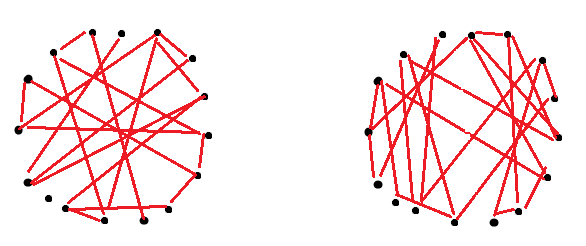
\includegraphics[scale=0.8]{graphs.png}
    \caption{On the left we have $G_{16, 1/2}$. On the right we have $G_{16, 1/2, 1/3}$. Definitely made with Matlab and not MS Paint.}
    \label{fig:graphs}
\end{figure}


%Given a \emph{non-trivial} monotone increasing property $\mathcal P_n$ of graphs on $n$ vertices (that is, $\mathcal P_n\neq \emptyset$), there must exist $0\leq m\leq \binom{n}{2}$ for which {\bf every} graph $G$ on $n$ vertices and with at least $m$ edges satisfies $\mathcal P_n$. Determining the minimal such $m$ for a specific property can be quite challenging and is a main theme of research in Extremal Graph Theory.

%In this paper we consider an analogous problem for random graphs which is about finding their probability \emph{threshold} behavior. Note that unlike the discussion above, for random graphs we are looking for the `first' moment for which {\bf most} of the graphs satisfy $\mathcal P_n$, and not all of them. More rigorously, a function $q(n)$ is a \emph{threshold function} for the property $\mathcal P_n$ if and only if,
%as $n$ goes to infinity,

In this paper we investigate how to identify the underlying communities in a realization of $G_{n, p, q}$. Of course, if we just randomly guess which community each vertex belongs to, then we expect to correctly classify around half of the vertices with high probability. If $p$ and $q$ are fixed constants, $p\neq q$, it turns out we can do much better.

\begin{theorem}
	Let $p\neq q$. Then with high probability we can correctly classify all but a constant number of vertices in a realization of $G_{n, p, q}$.
\end{theorem}

With a little bit of linear algebra, we address the case where $p$ and $q$ are allowed to depend on $n$.

\begin{theorem}
	Let $0\leq p,q \leq 1$ be such that $p-q = \frac{100}{\sqrt{n}}$. Then with high probability, we can correctly classify all but $\frac{288p}{(p-q)^2}$ vertices in a realization of $G_{n, p, q}$.
\end{theorem}

Our main tool for proving this result is a theorem due to Davis and Kahan.

\begin{theorem}
	Let $B$ and $M$ be symmetric matrices. Let $R = M-B$. Let $\alpha_i$ be the eigenvalues of $B$ with eigenvectors $v_i$ and $\mu_i$ of $M$ with corresponding eigenvectors $w_i$. Let $\theta_i$ be the angle between $v_i$ and $w_i$. Then
	\[
	\sin \theta_i \leq \frac{2\|R\|}{\min_{j\neq i}|\mu_i-\mu_j|}.
	\]
\end{theorem}

The rest of the paper is organized as follows...

\end{document} 